% FILE: decay-chains-diagonal-left-final-adjusted.tex
% This is a standalone file for the TikZ figure.
% MODIFIED: Adjusted chain spacing and implemented robust centering for the main title.
%injection should use implantation in specialized English scientific notation , but I am lazy.If code can work ,don't change it.
\documentclass[tikz, border={1cm 1cm 1cm 1cm}]{standalone} % Use the standalone class with tikz option

\usetikzlibrary{
    positioning,  % For placing nodes relative to each other
    arrows.meta,  % For modern arrow styles
    calc          % For calculating coordinates
}
\usepackage{amsmath} % For math symbols
\usepackage{ragged2e} % For \Centering command
%\usepackage{classico}

\begin{document}

% --- TikZ Picture Environment ---
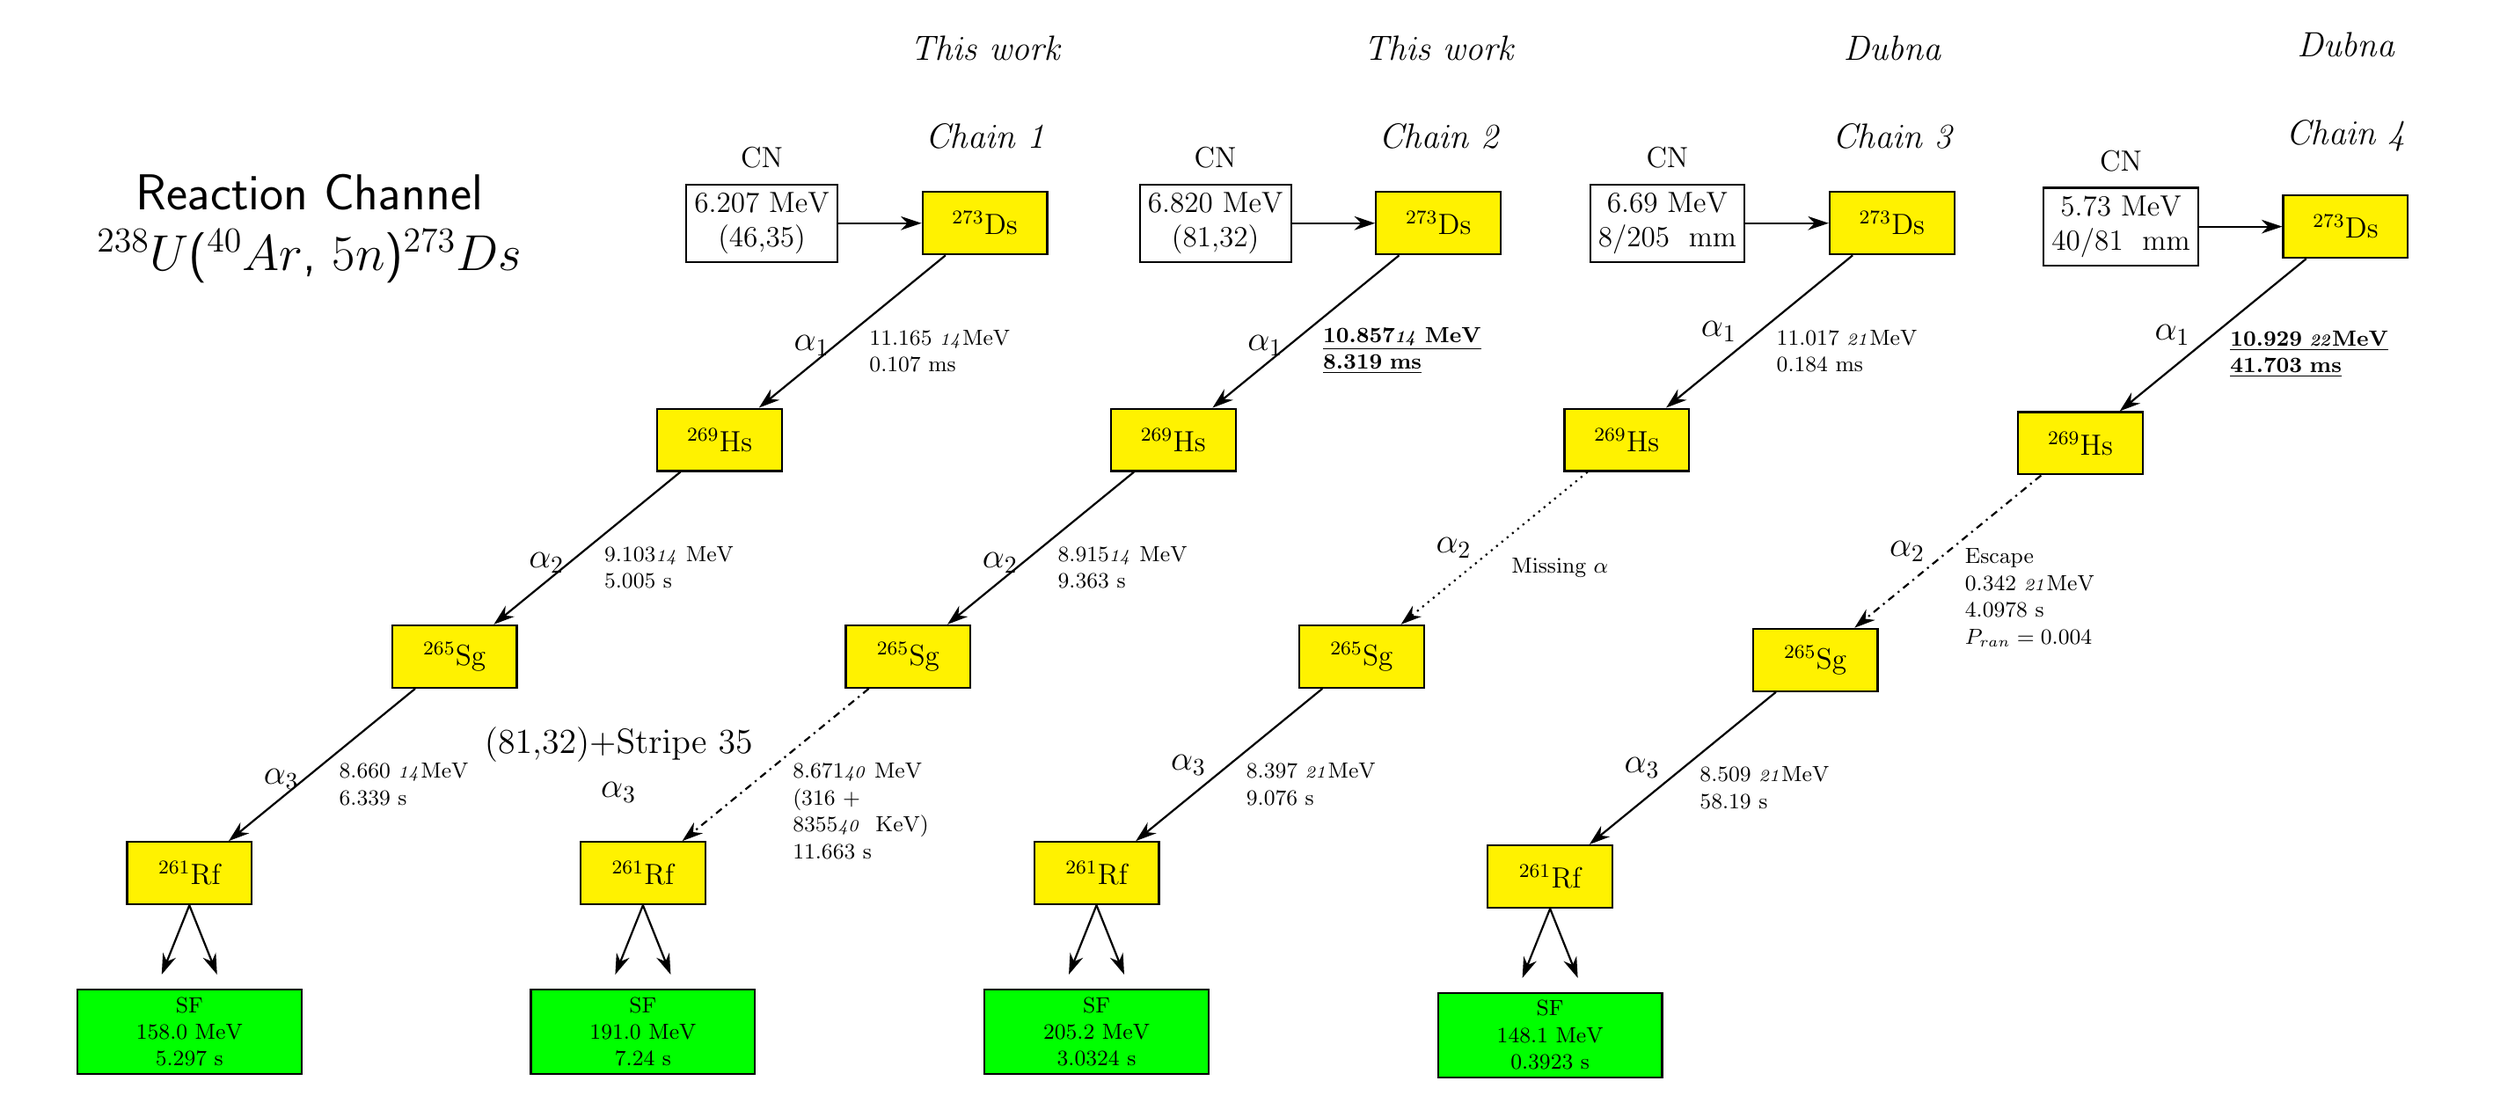
\begin{tikzpicture}

    % --- Style Definitions (for consistency and easy changes) ---
    \tikzset{
        nuclide/.style     = {rectangle, draw=black, thick, minimum height=0.9cm, minimum width=1.8cm, align=center, font=\large,fill=yellow},
        injection/.style   = {rectangle, draw=black, thick, minimum height=0.9cm, minimum width=1.8cm, align=center, font=\large}, % MODIFICATION: Added style for injection box
        decay/.style       = {-{Stealth[length=3mm, width=2mm]}, thick},
        alpha_label/.style = {font=\Large, align=center},
        prop_label/.style  = {font=\small, align=left, inner sep=1pt, text width=2.8cm, anchor=west}, 
        title/.style       = {font=\itshape\Large, align=center, text width=3.5cm},%\bfseries
        reaction/.style    = {font=\sffamily\huge, align=center, text width=8cm},
        sfinfo/.style      = {font=\small, align=center, text width=3cm, rectangle, draw=black, thick, minimum width=1.8cm, fill=green}
    }

    % --- Define key distances for easy layout tuning ---
    \def\diagvsep{2.2cm}    % Vertical separation between nuclides in a chain
    \def\diaghsep{2.0cm}    % Horizontal separation between nuclides in a chain
    % MODIFIED: Reduced horizontal separation between chains from 7.5cm to 6.8cm
    \def\chainhsep{2.8cm}   
    \def\sfbranchlen{1.0cm} % Length of the SF branch arrows

    % --- Chain 1 (IMP 1) ---
    \node[title] (title1) at (0,0) {\Centering This work\\~\\Chain 1};
    \node[nuclide, below=0.5cm of title1] (Ds1) {${}^{273}$Ds};
    
    % --- MODIFICATION START: Added injection box and arrow ---
    \node[injection, left=1.2cm of Ds1] (Inj1) {6.207 MeV \\(46,35) };
    \node[font=\large, above=0.1cm of Inj1] {CN};
    \draw[decay] (Inj1) -- (Ds1);
    % --- MODIFICATION END ---

    \node[nuclide, below left=\diagvsep and \diaghsep of Ds1] (Hs1) {${}^{269}$Hs};
    \node[nuclide, below left=\diagvsep and \diaghsep of Hs1] (Sg1) {${}^{265}$Sg};
    \node[nuclide, below left=\diagvsep and \diaghsep of Sg1] (Rf1) {${}^{261}$Rf};
    %\draw[decay] (Ds1) -- node[midway, left=0.2cm, alpha_label] { (46,35)\\$ \alpha_1$} node[midway, right=0.2cm, prop_label] {\\~\\ 11.165 {\scriptsize\textit{14}}MeV \\ 0.107 ms} (Hs1);
    \draw[decay] (Ds1) -- node[midway, left=0.2cm, alpha_label] { \\$ \alpha_1$} node[midway, right=0.2cm, prop_label] {\\~\\ 11.165 {\scriptsize\textit{14}}MeV \\ 0.107 ms} (Hs1);
    \draw[decay] (Hs1) -- node[midway, left=0.2cm, alpha_label] { \\$ \alpha_2$} node[midway, right=0.2cm, prop_label] {\\~\\ 9.103{\scriptsize\textit{14}} MeV \\ 5.005 s} (Sg1);
    \draw[decay] (Sg1) -- node[midway, left=0.2cm, alpha_label] { \\$ \alpha_3$} node[midway, right=0.2cm, prop_label] {\\~\\ 8.660 {\scriptsize\textit{14}}MeV \\ 6.339 s} (Rf1);
    \draw[decay] (Rf1.south) -- ++(-0.4, -\sfbranchlen);
    \draw[decay] (Rf1.south) -- ++(0.4, -\sfbranchlen);
    \node[sfinfo, below=\sfbranchlen+0.2cm of Rf1.south] {SF \\ 158.0 MeV \\ 5.297 s};
    % --- Chain 2 (IMP 2) ---
    \node[title, right=\chainhsep of title1] (title2) {\Centering This work\\~\\Chain 2};
    \node[nuclide, below=0.5cm of title2] (Ds2) {${}^{273}$Ds};

     % --- MODIFICATION START: Added injection box and arrow ---
    \node[injection, left=1.2cm of Ds2] (Inj2) {6.820 MeV \\(81,32) };
    \node[font=\large, above=0.1cm of Inj2] {CN};
    \draw[decay] (Inj2) -- (Ds2);
    % --- MODIFICATION END ---

    \node[nuclide, below left=\diagvsep and \diaghsep of Ds2] (Hs2) {${}^{269}$Hs};
    \node[nuclide, below left=\diagvsep and \diaghsep of Hs2] (Sg2) {${}^{265}$Sg};
    \node[nuclide, below left=\diagvsep and \diaghsep of Sg2] (Rf2) {${}^{261}$Rf};
    \draw[decay] (Ds2) -- node[midway, left=0.2cm, alpha_label] {\\$\alpha_1$} node[midway, right=0.2cm, prop_label] {\\~\\ \underline{\textbf{10.857{\scriptsize\textit{14}} MeV}} \\ \underline{\textbf{8.319 ms}}} (Hs2);
    \draw[decay] (Hs2) -- node[midway, left=0.2cm, alpha_label] {\\$\alpha_2$} node[midway, right=0.2cm, prop_label] {\\~\\ 8.915{\scriptsize\textit{14}} MeV \\ 9.363 s} (Sg2);
    \draw[decay,dash dot] (Sg2) -- node[midway, left=0.2cm, alpha_label] {(81,32)+Stripe 35\\$\alpha_3$} node[midway, right=0.2cm, prop_label] {\\~\\~\\ ~\\8.671{\scriptsize\textit{40}} MeV \\ (316 + 8355{\scriptsize\textit{40}}~ KeV)  \\ 11.663 s} (Rf2);
    \draw[decay] (Rf2.south) -- ++(-0.4, -\sfbranchlen);
    \draw[decay] (Rf2.south) -- ++(0.4, -\sfbranchlen);
    \node[sfinfo, below=\sfbranchlen+0.2cm of Rf2.south] {SF \\ 191.0 MeV \\ 7.24 s};
    % --- Chain 3 (Dubna 1) ---
    \node[title, right=\chainhsep of title2] (title3) {\Centering Dubna \\~\\Chain 3};
    \node[nuclide, below=0.5cm of title3] (Ds3) {${}^{273}$Ds};

    % --- MODIFICATION START: Added injection box and arrow ---
    \node[injection, left=1.2cm of Ds3] (Inj3) {6.69 MeV \\8/205 ~mm };
    \node[font=\large, above=0.1cm of Inj3] {CN};
    \draw[decay] (Inj3) -- (Ds3);
    % --- MODIFICATION END ---

    \node[nuclide, below left=\diagvsep and \diaghsep of Ds3] (Hs3) {${}^{269}$Hs};
    \node[nuclide, below left=\diagvsep and \diaghsep of Hs3] (Sg3) {${}^{265}$Sg};
    \node[nuclide, below left=\diagvsep and \diaghsep of Sg3] (Rf3) {${}^{261}$Rf};
    \draw[decay] (Ds3) -- node[midway, left=0.2cm, alpha_label] {$\alpha_1$} node[midway, right=0.2cm, prop_label] {\\~\\ 11.017 {\scriptsize\textit{21}}MeV \\ 0.184 ms} (Hs3);
    \draw[decay,dotted] (Hs3) -- node[midway, left=0.2cm, alpha_label] {$\alpha_2$} node[midway, right=0.2cm, prop_label] {\\~\\ Missing $\alpha$} (Sg3);
    \draw[decay] (Sg3) -- node[midway, left=0.2cm, alpha_label] {$\alpha_3$} node[midway, right=0.2cm, prop_label] {\\~\\ 8.397 {\scriptsize\textit{21}}MeV \\ 9.076 s} (Rf3);
    \draw[decay] (Rf3.south) -- ++(-0.4, -\sfbranchlen);
    \draw[decay] (Rf3.south) -- ++(0.4, -\sfbranchlen);
    \node[sfinfo, below=\sfbranchlen+0.2cm of Rf3.south] {SF \\ 205.2 MeV \\ 3.0324 s};
    % --- Chain 4 (Dubna 2) ---
    \node[title, right=\chainhsep of title3] (title4) {\Centering Dubna \\~\\Chain 4};
    \node[nuclide, below=0.5cm of title4] (Ds4) {${}^{273}$Ds};

    \node[injection, left=1.2cm of Ds4] (Inj4) {5.73 MeV \\40/81 ~mm };
    \node[font=\large, above=0.1cm of Inj4] {CN};
    \draw[decay] (Inj4) -- (Ds4);

    \node[nuclide, below left=\diagvsep and \diaghsep of Ds4] (Hs4) {${}^{269}$Hs};
    \node[nuclide, below left=\diagvsep and \diaghsep of Hs4] (Sg4) {${}^{265}$Sg};
    \node[nuclide, below left=\diagvsep and \diaghsep of Sg4] (Rf4) {${}^{261}$Rf};
    \draw[decay] (Ds4) -- node[midway, left=0.2cm, alpha_label] {$\alpha_1$} node[midway, right=0.2cm, prop_label] {\\~\\ \underline{\textbf{10.929 {\scriptsize\textit{22}}MeV}} \\ \underline{\textbf{41.703 ms}}} (Hs4);
    \draw[decay,dash dot] (Hs4) -- node[midway, left=0.2cm, alpha_label] {$\alpha_2$} node[midway, right=0.2cm, prop_label] {\\~\\~\\~\\ Escape\\0.342 {\scriptsize\textit{21}}MeV  \\ 4.0978 s\\$P_{ran}=0.004$} (Sg4);
    \draw[decay] (Sg4) -- node[midway, left=0.2cm, alpha_label] {$\alpha_3$} node[midway, right=0.2cm, prop_label] {\\~\\ 8.509 {\scriptsize\textit{21}}MeV \\ 58.19 s} (Rf4);
    \draw[decay] (Rf4.south) -- ++(-0.4, -\sfbranchlen);
    \draw[decay] (Rf4.south) -- ++(0.4, -\sfbranchlen);
    \node[sfinfo, below=\sfbranchlen+0.2cm of Rf4.south] {SF \\ 148.1 MeV \\ 0.3923 s};
    % --- Centered Reaction Channel Text at the top ---
    % MODIFIED: This new positioning robustly centers the title over the entire drawing
    % by calculating the midpoint between the far left of the first chain (Ds1.west)
    % and the far right of the last chain (Rf4.east).
    \node[reaction, anchor=north west] at ($(title1.north west) + (-12cm, -2cm)$) {
        Reaction Channel\\ ${}^{238}U$(${}^{40}Ar$, $5n$)${}^{273}Ds$
    };
\end{tikzpicture}
\end{document}